\documentclass[a4paper,11pt]{article}
\usepackage{amsmath, amssymb, amsthm, amsfonts, mathtools}
\usepackage[utf8]{inputenc}
\usepackage[T1]{fontenc}
\usepackage{comment}
\usepackage{marginnote}
\usepackage{booktabs}
\usepackage{tikz, tikz-cd}
\usepackage{hyperref}
\usepackage{geometry}
\usepackage[english, ngerman]{babel}
\usepackage{csquotes}
\usepackage[backend=biber, style=numeric, sorting=none]{biblatex}
\usepackage{BA_Titelseite}

%Namen des Verfassers der Arbeit
\author{Paul Jin Robaschik}
%Geburtsdatum des Verfassers
\geburtsdatum{25. Juni 2004}
%Gebortsort des Verfassers
\geburtsort{K\"oln}
%Datum der Abgabe der Arbeit
\date{\today}

%Name des Betreuers
% z.B.: Prof. Dr. Peter Koepke
\betreuer{Betreuer: Prof. Dr. Markus Hausmann}
%Name des Zweitgutachters
\zweitgutachter{Zweitgutachterin: Dr. Elizabeth Tatum}
%Name des Instituts an dem der Betreuer der Arbeit t�tig ist.
%z.B.: Mathematisches Institut
\institut{Mathematisches Institut}
%\institut{Institut f\"ur Angewandte Mathematik}
%\institut{Institut f\"ur Numerische Simulation}
%\institut{Forschungsinstitut f\"ur Diskrete Mathematik}
%Titel der Bachelorarbeit
\title{Bordism Homology and Cohomology}
%Do not change!
\ausarbeitungstyp{Bachelorarbeit Mathematik}


\newtheorem{definition}{Definition}[section]
\newtheorem{theorem}[definition]{Theorem}
\newtheorem*{remark}{Remark}
\newtheorem{proposition}[definition]{Proposition}
\newtheorem{lemma}[definition]{Lemma}
\newtheorem{corollary}[definition]{Corollary}
\newtheorem*{example}{Example}
\newtheorem*{nonex}{Non-example}


\newcommand{\demph}[1]{{\underline{{\textbf{#1}}}}}
\newcommand{\restrict}[1]{_{|_{#1}}}
\def\R{\mathbb{R}}

\addbibresource{sources.bib}

\begin{document}
\maketitle
\selectlanguage{english}
\tableofcontents\newpage

\begin{comment}
\newgeometry{
	left=20mm, % left margin
    top=25mm,
    right=20mm, % right margin
	%textwidth=150mm, % main text block
	%marginparsep=5mm, % gutter between main text block and margin notes
	%marginparwidth=40mm, % width of margin notes
  bmargin=2cm % height of foot note space
}
\end{comment}

\setcounter{section}{-1}

\section{Introduction/Motivation}
%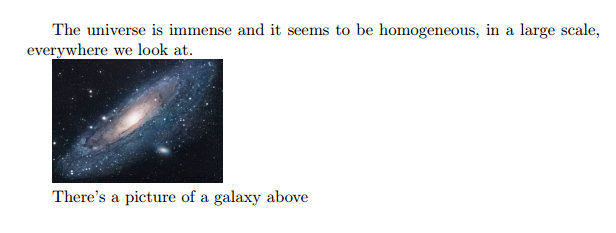
\includegraphics{galaxy.png}

Recall the definition of homotopy groups \(\pi_n(X)\) as the set of homotopy classes of maps from the \(n\)-sphere \(S^n\) to a space \(X\). 
The problem with homotopy groups is that they are, in general, hard to compute, even for simple spaces such as spheres. 

The general idea of bordism is to replace the \(n\)-sphere with a manifold of dimension \(n\) and to consider the homotopy classes of maps from this manifold to a space \(X\).

Testing citations:\cite{atiyah},\cite{brocker},\cite{thom},\cite{lee},\cite{hatcher},\cite{dieck},\cite{luck}

\section{Bordism}

\subsection{Manifolds}

\begin{definition}[Topological manifold\ {\cite[pp.2-3]{lee}}]
    An \(n\)-dimensional \demph{topological manifold} is a topological space \(M\) such that:
    \begin{itemize}
        \item \(M\) is Hausdorff, (i.e.\ any two distinct points can be separated by disjoint open sets),
        \item \(M\) is second countable, (i.e.\ there exists a countable basis for the topology of \(M\)),
        \item \(M\) is locally Euclidean (i.e.\ every point in \(M\) has a neighbourhood homeomorphic to an open subspace of \(\mathbb{R}^n\)).
    \end{itemize}
    We will often write \(M^n\) for an \(n\)-dimensional manifold.
\end{definition}

\begin{example}
    \(\mathbb{R}^n\) is an \(n\)-dimensional topological manifold.
\end{example}

\begin{example}\label{sphere chart}
    The \(n\)-dimensional sphere \(S^n\) is an \(n\)-dimensional topological manifold. Hausdorffness and second countability follow from \(S^n\subset \mathbb{R}^{n+1}\). For local Euclideanness, we can use the local charts \[\varphi_i^\pm:U_i:=\{(x_0,\dots,x_n)\in S^n\mid \pm x_i>0\}\to B_1^n(0)\] by \[(x_0,\dots,x_i,\dots,x_n)\mapsto(x_0,\dots,x_{i-1},x_{i+1},\dots,x_n)\]
\end{example}

\begin{nonexs}
    %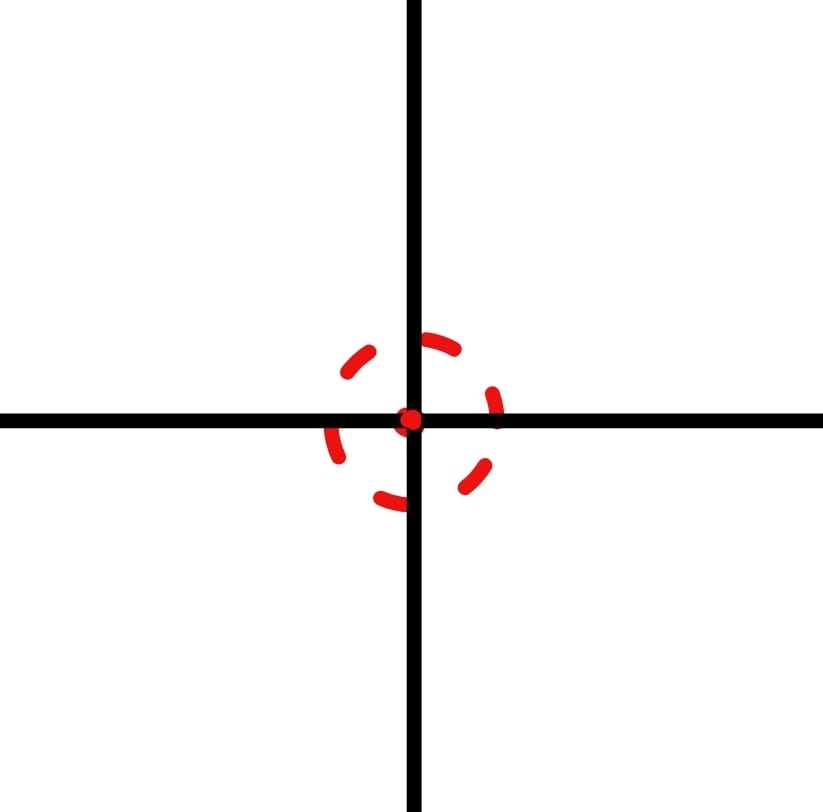
\includegraphics[width=0.2\textwidth]{cross}
    \begin{itemize}
        \item Two crossing lines in \(\mathbb{R}^2\) are not a topological manifold, because they are not locally Euclidean at the crossing point. 
        \item The line with two origins is not a topological manifold. It is not Hausdorff, as the two origins cannot be separated by disjoint open sets.
        \item \(\coprod_{i\in \mathbb{R}}\{pt\}\) is not a topological manifold, because it is not second countable, as it has uncountably many connected components.
        \item \(S^1\amalg\{pt\}\) is not a topological manifold, because it is, depending on the point, locally homeomorphic to \(\mathbb{R}^2\) or \(\mathbb{R}\), and the dimension needs to be fixed.
    \end{itemize}
\end{nonexs}

\begin{remark}
    One could replace the condition of being second countable with the condition of being paracompact (i.e.\ every open cover of \(M\) admits a locally finite refinement). The following equivalence holds:
    \[\text{second countable}\iff \text{paracompact and countably many connected components}\]
    %This is shown in\ \cite{lee}. --- It is not :(
\end{remark}

%Being a topological manifold is just a property of a topological space \(M\). We will give manifolds extra structure by defining a smooth structure on them.

\begin{definition}[(Smooth) Atlas\ {\cite[p.12]{lee}}]
    Let \(M\) be a topological manifold. A \demph{(smooth) atlas} \(\mathcal{A}\) on \(M\) is a collection of smooth charts \((U_\alpha,\varphi_\alpha)\) such that:
    \begin{itemize}
        \item the \(\{U_\alpha\}\) cover \(M\),
        \item the charts are pairwise smoothly compatible (i.e.\ the transition functions \(\varphi_j \circ \varphi_i^{-1}:\varphi_i(U_i\cap U_j)\to\varphi_j(U_i\cap U_j)\) are smooth)
    \end{itemize}
\end{definition}

\begin{example}
    The charts we chose for the \(n\)-sphere \(S^n\) in \ref{sphere chart} form a smooth atlas on \(S^n\).
\end{example}

\begin{definition}[Equivalence of atlases]
    Two atlases \(\mathcal{A}\) and \(\mathcal{A}^\prime\) (on a fixed topological manifold) are said to be \demph{equivalent}, if their union is still on atlas.
\end{definition}

It can be shown that this is indeed an equivalence relation, but I will omit the proof here.

\begin{definition}[Smooth manifold\ {\cite[p.13]{lee}}]
    A \demph{smooth manifold} \(M=(M,[\mathcal{A}])\) consists of
    \begin{itemize}
        \item a topological manifold \(M\),
        \item an equivalence class \([\mathcal{A}]\) of smooth atlases on \(M\).
    \end{itemize}
\end{definition}

\begin{example}
    The \(n\)-sphere \(S^n\) with the atlas given by the charts in \ref{sphere chart} is a smooth manifold.
\end{example}

\begin{example}[Subset of manifolds]
    For a manifold \(M,[\mathcal{A}]\) any open subset is a manifold. The atlas is given by restriction of the charts in \([\mathcal{A}]\) to the open subset.
\end{example}

\begin{example}[Product of manifolds]
    For manifolds \(M,N\), \(M\times N\) is a manifold with the charts\[\{(U\times V,(\varphi,\psi))\mid(U,\varphi),(V,\psi)\text{ charts of }M,N\}\].
\end{example}

\begin{remark}
    While being a topological manifold is just a property of the topological space \(M\), begin a smooth manifold gives the manifold extra structure.
\end{remark}

\begin{example}
    \(\mathbb{R},[(\mathbb{R},\mathrm{id})]\) and \(\mathbb{R},[\mathbb{R},x\mapsto x^3]\) are two different smooth manifolds, because the transition functions between them are not smooth: \(\mathrm{id}\circ(x\mapsto x^3)^{-1}=(x\mapsto x^{\frac13})\).
\end{example}

\begin{definition}[Manifold with boundary\ {\cite[p.25]{lee}}]
    To get a definition of a (smooth or topological) \demph{manifold with boundary}, replace the condition of the manifold being locally Euclidean with the condition that every point has a neighbourhood homeomorphic to an open subspace of \(\mathbb{H}^n:=\{(x_1,\dots,x_n)\in\mathbb{R}\mid x_1\geq0\}\) (the half space).
\end{definition}

\begin{comment}
\begin{definition}[Manifold]
    A \demph{smooth manifold with boundary} \(M=(M,[\mathcal{A}])\) is the data of a topological space \(M\) and an equivalence class \([\mathcal{A}]\) of smooth atlases such that:
    \begin{itemize}
        \item \(M\) is Hausdorff,
        \item \(M\) is second countable,
        \item \(\mathcal{A}\) is locally finite.
    \end{itemize}
\end{definition}
\end{comment}

\begin{remark}
    In this thesis, with \demph{manifold} we will always mean a smooth manifold with boundary.
\end{remark}

\begin{definition}[Boundary\ {\cite[p.25]{lee}}]
    A point \(x\in M^n\) is called a \demph{interior point} if it admits a neighbourhood homeomorphic to \(\mathbb{R}^n\). Otherwise, it is called a \demph{boundary point}. The set of boundary points is denoted by \(\partial M\) and is called the \demph{boundary} of \(M\).\\
    If a manifold is compact and has empty boundary, it is called a \demph{closed manifold}. %If a manifold is compact and has non-empty boundary, it is called a \demph{compact manifold with boundary}. If a manifold is not compact, it is called an \demph{open manifold}
\end{definition}

\begin{example}
    \(([0,1],[([0,1],i)])\), where \(i\) is the inclusion into \(\mathbb{R}\), is a 1-manifold. Its boundary is \(\partial [0,1]=\{0,1\}\).
\end{example}

\begin{example}
    \(\mathbb{H}^n\) is a manifold with boundary \(\mathbb{R}^{n-1}\)
\end{example}

\begin{example}
    The \(n\)-disk \(D^n\) is a manifold with boundary \(S^{n-1}\)
\end{example}

\begin{remark}
    The boundary of an \(n\)-dimensional manifold is an \((n-1)\)-dimensional submanifold.
\end{remark}

%\section{Bordism}

The problem with working with manifolds is that they are hard to classify up to homeomorphism or diffeomorphism. Bordism is a way to classify manifolds up to a weaker equivalence relation, which is easier to work with.

\subsection{Unoriented bordism}
\subsubsection{Definitions}
Examples need to be added here, too.

\begin{definition}[Singular manifold\ {\cite[II, Definition 1.1]{brocker}}]\label{singular manifold}
    Let \(X\) be a topological space. An \(n\)-dimensional \demph{singular manifold} in \(X\) is a pair \(M,f\) of a compact manifold \(M^n\) and a continuous map \(f:M\to X\).\\
    The \demph{boundary} of a singular manifold is \(\partial(M,f):=(\partial M, \partial f):=(\partial M,f\restrict{\partial M})\).
\end{definition}

\begin{definition}[Nullbordant\ {\cite[II, Definition 1.2]{brocker}}]
    Let \((M,f)\) be a singular manifold in \(X\). We say that \((M,f)\) is \demph{nullbordant}, if there exists a singular manifold \((B,F)\), such that \(\partial(B,F)=(M,f)\).

    \(B,F\) is then called a \demph{nullbordism} of \((M,f)\).
\end{definition}

\begin{example}
    For \(X\) the point space, and \(M=S^n\), we have a nullbordism \(B=D^{n+1}\).
\end{example}

\begin{example}
    For \(X\) the point space, and \(M=\mathbb{T}^1\) the torus, \(S^1\times D^2\), the filled torus, is a nullbordism.
\end{example}

\begin{example}
    For \(M=\emptyset\), any closed manifold is a nullbordism of \(M\), no matter what the space \(X\) is.
\end{example}

\begin{example}
    \(X=S^1\), \(M=S^1\), and \(f\) is given by wrapping around the circle twice, a nullbordism is given by the M\"obius strip \(\mathbb{M}\) with \(F\) as projection onto the circle.
\end{example}
Draw a picture.

\begin{definition}[Bordant\ {\cite[II, Definition 1.3]{brocker}}]\label{bordant}
    Let \((M,f)\) and \((N,g)\) be singular manifolds in \(X\). We say that \((M,f)\) and \((N,g)\) are \demph{bordant}, if their sum \((M,f)+(N,g):=(M+N, (f,g)):=(M\amalg N, f\amalg g)\) is nullbordant.

    A nullbordism of \((M,f)+(N,g)\) is called a \demph{bordism} between \((M,f)\) and \((N,g)\).
\end{definition}

We will refer to this relation as \demph{bordism relation}.

\begin{remark}
    \[(M,f)+(\emptyset,g) \text{ are bordant} \iff (M,f) \text{ is nullbordant}\]
\end{remark}

\begin{example}[Cylinder]\label{cylinder bordism}
    For an arbitrary \(X\), and \((M_1,f_1)=(M_2,f_2)\), we always get the cylinder as a bordism: \((M\times[0,1],f\circ\mathrm{pr}_1)\).
\end{example}
Draw a picture

\begin{example}[Pair of pants]
    For \(X=\mathrm{pt}\), \((M_1,f_1)=(M,f)\amalg (M,f)\) and \(M_2=M\# M\).
\end{example}
Look this up again. Maybe it suffices to take \(X\) path-connected. Draw a picture.

\begin{nonex}
    \(\mathrm{pt}\) and \(\mathrm{pt}\amalg\mathrm{pt}\) are not bordant, as \(1\)-manifolds either have 2 or 0 boundary points.
\end{nonex}
Draw a picture.

\begin{proposition}\cite[II, Satz 1.4]{brocker}
    Being bordant is an equivalence relation on the set of singular manifolds.
\end{proposition}

\begin{proof}\cite{brocker}, \cite[p.8]{conner}
    \begin{itemize}
        \item Symmetry: Follows from the symmetry of the disjoint union. If \((M,f)\) and \((N,g)\) are bordant, then there exists a nullbordism of \((M,f)+(N,g)=(M\amalg N, f\amalg g) = (N\amalg M, g\amalg f) = (N,g)+ (M,f)\). So, a bordism between \((M,f)\) and \((N,g)\) is also bordism between \((N,g)\) and \((M,f)\).
        \item Reflexivity: We have already constructed a bordism between \(M,f\) and itself In\ \ref{cylinder bordism}.
        \item Transitivity: Let \(B_1,F_1\) be the bordism between \(M_1,f_1\) and \(M_2,f_2\), and let \(B_2,F_2\) be the bordism between \(M_2,f_2\) and \(M_3,f_3\). Then we can \enquote{glue} the two bordisms together at the common boundary \(M_2,f_2\). We only need to check that the gluing is smooth, i.e. \((B_1,F_1)\cup_{(M_2,f_2)}(B_2,F_2)\) is a smooth manifold. We can find a collar of \(M_2\) in both \(B_1\) and \(B_2\). These collars glued together are homeomorphism to \(M_2\times(-1,1)\). This induces a smooth structure on the glued collar, and let \(B\setminus M_2\) inherit the smooth structure from \(B_1\) and \(B_2\). Then there exists a smooth structure on \(B\) by a previous lemma.
    \end{itemize}
\end{proof}
Draw a picture.
Need to add collar theorem somewhere up.
and inducing structure.

Check smooth structure!

\begin{definition}[bordism group\ {\cite[II, Definition 1.5]{brocker}}]
    The equivalence classes of the bordism relation are called \demph{bordism classes} and are denoted by \([M,f]\).
    The set of bordism classes of \(n\)-dimensional singular manifolds in \(X\) is denoted by \(\mathfrak{N}_n(X)\) and is called the \(n\)\demph{-th bordism group of }\(X\).
    \[\mathfrak{N}_n=\{\text{singular \(n\)-manifolds in \(X\)}\}\big/\text{bordism}\]
\end{definition}

Observe the similarity with the definition of singular homology groups: We defined the singular homology groups as the quotient of kernel and image of some maps. Here, the same thing happens: Our map here is the boundary map.

\begin{theorem}\ \cite[II, Satz 2.1]{brocker}
    The bordism groups are abelian groups with the operation defined in\ \ref{bordant}:
    \[[M_1,f_1]+[M_2,f_2]=[M_1+M_2,(f_1,f_2)]\]
    Every element in this group has order at most \(2\), making \(\mathfrak{N}_n(X)\) a \(\mathbb{F}_2\)-vector space.
\end{theorem}

\begin{proof}
    \ \cite{brocker}
    The neutral element is the bordism class of the empty manifold (i.e.\ the class of all nullbordant manifolds).\\
    \enquote{+} is associative and commutative, because the disjoint union is associative and commutative.\\
    It is well-defined: by + of the two bordisms.\\
    Since being bordant is a reflexive, every element is its own inverse.
\end{proof}

Let \(X,Y\) be two topological spaces. Then we define a product map
\[\cdot:\mathfrak{N}_p(X)\times\mathfrak{N}_q(Y)\to\mathfrak{N}_{p+q}(X\times Y)\]
as
\[((M,f),(N,g))\mapsto (M\times N,f\times g)\]

\begin{remark}
    Check: Well-definedness, bilinearity
\end{remark}

For \(X=\{\mathrm{pt}\}\), we write \(\mathfrak{N}_n(X)\) as \(\mathfrak{N}_n\) and for elements of \(\mathfrak{N}_n\), we will omit the map from the notation (\([M]=[M,f]\)).

\begin{definition}[graded bordism ring\ {\cite[Satz 2.2]{brocker}}]
    \[\mathfrak{N}_\ast:=\bigoplus_{n\in\mathbb{Z}}\mathfrak{N}_n\]
    is a graded ring over \(\mathbb{F}_2\) and is called the \demph{bordism ring}.
\end{definition}

\begin{remark}
    As \(\mathbb{F}_2\) is a field, \(\mathfrak{N}_\ast\) is a graded vector space over \(\mathbb{F}_2\).
\end{remark}

Maybe do a quick check.

\begin{definition}[graded bordism module\ {\cite[Satz 2.3]{brocker}}]
    \[\mathfrak{N}_\ast(X):=\bigoplus_{n\in\mathbb{Z}}\mathfrak{N}_n(X)\]
    is a graded module over \(\mathfrak{N}_\ast\) via
    \[[M]\cdot[N,f]=[M\times N, f\circ \mathrm{pr}_2]\]
    where \(\mathrm{pr}_2:M\times N\to N\) is the projection onto the second factor.
\end{definition}

\begin{remark}
    Notice that in this definition, this is a right module, but since we could just project to the first factor instead, we also get a left module structure.
\end{remark}

\subsubsection{The Eilenberg-Steenrod axioms}\label{es axioms}
The Eilenberg-Steenrod axioms are a set of axioms that characterize the homology and cohomology theories.

\begin{definition}[Homology theory\ {\cite[Definition 1.1]{luck}}]
    A \demph{homology theory} \(\mathcal{H}_\ast=(\mathcal{H}_\ast,\partial_\ast)\) with coefficients in \(R\)-modules is a covariant functor\[\mathcal{H}_\ast:\mathrm{TOP}^2\to\mathbb{Z}\text{-graded }R\text{-modules}\]
    together with a natural transformation \[\partial_\ast:\mathcal{H}_\ast\to\mathcal{H}_{\ast-1}\circ I\]
    
    \begin{itemize}
        \item \textbf{Homotopy invariance}\\
        Let \(f,g:(X,A)\to(Y,B)\) be homotopic maps. Then for all \(n\in\mathbb{Z}\), we have
        \[\mathcal{H}_n(f)=\mathcal{H}_n(g):\mathcal{H}_n(X,A)\to\mathcal{H}_n(Y,B)\]
        \item \textbf{Long exact sequence}\\
        Let \((X,A)\) be a pair of spaces. Then for all \(n\in\mathbb{Z}\), we have the long exact sequence of homology groups:
        \begin{align*}
            \dots\xrightarrow{\partial_{n+1}(X,A)}\mathcal{H}_n(A)\xrightarrow{\mathcal{H}_n(i)}\mathcal{H}_n(X)\xrightarrow{\mathcal{H}_n(j)}\mathcal{H}_n(X,A)\xrightarrow{\partial_n(X,A)}\mathcal{H}_{n-1}(A)\to\dots
        \end{align*}
        \item \textbf{Excision}\\
        Let \(A\subset B\subset X\) be subspaces of \(X\) such that \(\overline{A}\subset B^\circ\). Then the inclusion \(i:(X\setminus B,A\setminus B)\to(X,A)\) induces an isomorphism of homology groups for all \(n\in\mathbb{Z}\):
        \[\mathcal{H}_n(i):\mathcal{H}_n(X\setminus A, B\setminus A)\xrightarrow{\cong}\mathcal{H}_n(X,B)\]
    \end{itemize}
    Sometimes one adds the following axioms:
    \begin{itemize}
        \item \textbf{Disjoint union axiom}\\
        Let \({\{X_i\}}_{i\in I}\) be a family of topological spaces. Let \(j_i:X_i\to\coprod_{i\in I}X_i\) be the inclusion. Then for all \(n\in\mathbb{Z}\), we have a bijection:
        \[\bigoplus_{i\in I}\mathcal{H}_n(j_i):\bigoplus_{i\in I}\mathcal{H}_n(X_i)\xrightarrow{\cong}\mathcal{H}_n\left(\coprod_{i\in I}X_i\right)\]
        \item \textbf{Dimension axiom}\\
        For the point space \(\mathrm{pt}\), we have
        \[\mathcal{H}_n(\mathrm{pt})\cong\begin{cases}R&n=0\\\{0\}&n\neq0\end{cases}\]
        
    \end{itemize}
    For homology theories, the abbreviation \(\mathcal{H}_\ast\) is often used to refer to \(\mathcal{H}_\ast(\{\mathrm{pt}\},\emptyset)\).
\end{definition}

Before we can say that bordism defines a homology theory, we need to define relative bordism.

\subsubsection{Relative bordism}

\begin{definition}[relative bordism\ {\cite[pp.524-525]{dieck}}]
    For a pair of topological spaces \((X,A)\), we call a \((M,f)=(M,\partial M,f)\) a \demph{singular manifold in }\(X\), if \(f:(M,\partial M)\to (X,A)\) is a continuous map of pairs.\\
    Two singular manifolds \((M_0,f_0)\) and \((M_1,f_1)\) in \(X\) are called \demph{bordant}, if there exists a singular manifold \((B,F)\) in \(X\), such that:
    \begin{itemize}
        \item \((B,F)\) is a (\(n+1\))-dimensional compact manifold with boundary,
        \item \(\partial B=\partial_0B\cup\partial_1B\cup\partial_2B\) such that \\
                \(\partial(\partial_2B)=\partial(\partial_0B)\amalg\partial(\partial_1B)\) and
                for \(i\in\{0,1\}\), \(\partial_i B\cap\partial_2B=\partial(\partial_i B)\)
        \item There are diffeomorphisms \(g:(M_i,f_i)\xrightarrow{\cong}(\partial_{i} B,\partial(\partial_{i}B))\) for \(i\in\{0,1\}\) such that \(\partial F\circ g_i=\partial f_i\)\\
        \(\partial f_i, \partial g_i, \partial F_i\) are as defined in\ \ref{singular manifold}.
        \item \(F(\partial_2B)\subseteq A\)
    \end{itemize}
    As before, \(B,F\) will be called a \demph{bordism} between \((M_0,f_0)\) and \((M_1,f_1)\) and a \demph{nullbordism} of \(M_0,f_0\) if \(M_1=\emptyset\).
\end{definition}

\begin{example}
    Disks on sphere
\end{example}

\begin{theorem}\cite[p.525]{dieck}
    Relative bordism is an equivalence relation on the set of singular manifolds in \(X\).
\end{theorem}

Maybe do a proof or just say that it is similar to the proof of the bordism relation.


relative bordism groups are graded modules in the same way. They are denoted by \(\mathfrak{N}_\ast(X,A)\).
If \(A=\emptyset\), the definition coincides with the definition of bordism groups.

\begin{lemma}\label{almost excision}\cite[Lemma 5.1]{zhang}, maybe \cite[21.1.8]{dieck}
    Let \([M,f]\in\mathfrak{N}_n(X,A)\) and \(V\) a embedded submanifold, such that \([V,f\restrict{V}]\in\mathfrak{N}_n(X,A)\) and \(f(M\setminus N)\subseteq A\). Then \([M,f]=[V,f\restrict{V}]\) in \(\mathfrak{N}_n(X,A)\).
\end{lemma}

\begin{proof}\cite{zhang}, maybe \cite{dieck}
    We need to show that \((M,f)\) and \((N,f\restrict{N})\) are bordant.\\
    Let \(B=M\times I\) the cylinder. \(\partial B= \underbrace{M\times\{0\}}_{M_0}\cup \underbrace{M\times\{1\}}_{M_1}\cup \partial M\times I\). Define \(g:B\to X\) as \(g(p,t)=f(p)\).\\
    Writing \(M_1=(M_1\setminus N_1)\cup N_1\), we get that \(M\times I\) is a bordism between \(M\) and \(N\), because
    \[g(\partial B\setminus(M_0\cup N_1))=g((M_1\setminus N_1)\cup(\partial M\times I))=f(M\setminus N)\cup f(\partial M)\subseteq A\]
\end{proof}

\subsubsection{Bordism homology}

\begin{lemma}\cite[II, Satz 3.2]{brocker}\label{functoriality}
    Relative bordism is a covariant functor \[\mathfrak{N}_\ast:\mathrm{TOP}^2\to\text{graded \(\mathfrak{N}_\ast\)modules}\]
\end{lemma}

\begin{proof}\cite{brocker} 
    Let \((X,A)\in\mathrm{Ob}(\mathrm{TOP}^2)\), we already saw
    \[(X,A)\xmapsto{\mathfrak{N}_\ast}\mathfrak{N}_\ast(X,A)\]
    For a map \(\mathrm{Mor}(\mathrm{TOP}^2)\ni f:(X,A)\to(Y,B)\), we take the induced map on the bordism groups:
    \[f_\ast:=\mathfrak{N}_\ast(f):\mathfrak{N}_\ast(X,A)\to\mathfrak{N}_\ast(Y,B)\]
    given by \(f_\ast[M,g]=[M,f\circ g]\) for \([M,g]\in\mathfrak{N}_n(X,A)\) and \(n\in\mathbb{N}\).\\
    Then we get that \(\mathfrak{N}_\ast(\mathrm{id}_{(X,A)})=\mathrm{id}_{\mathfrak{N}_\ast(X,A)}\) and for \(f:(X,A)\to(Y,B), g:(Y,B)\to(Z,C)\), we have for any \([M,h]\in\mathfrak{N}_\ast(X,A)\):
    \[{(g\circ f)}_{\ast}[M,h]=[M,g\circ f\circ h]=g_\ast[M,f\circ h]=g_\ast\circ f_\ast[M,h]\]
\end{proof}

\begin{lemma}[Naturality of the boundary map]
    The following diagram commutes: (Diagrams cannot be compiled for some reason)
    \begin{center}
        \begin{tikzcd}
            {\mathfrak{N}_n(A)} \arrow[r]& {\mathfrak{N}_{n-1}(X,A)}
        \end{tikzcd}
    \end{center}
\end{lemma}

\begin{proof}
    Let \([M,g]\in\mathfrak{N}_n(X,A)\). This maps to \([\partial M,g\restrict{\partial M}]\in\mathfrak{N}_{n-1}(A)\).
    Now \({f\restrict{A}}_\ast([\partial M,g\restrict{\partial M}])=[\partial M,f\circ g\restrict{\partial M}]\in \mathfrak{N}_{n-1}(B)\).\\
    On the other side, \((\partial\circ f_\ast)[M,g]=\partial [M,f_\ast\circ g]=[\partial M,(f_\ast\circ g)\restrict{\partial M}]\in \mathfrak{N}_{n-1}(B)\), which is the same as the previous composition, hence,
    \[\partial\circ f_\ast={f\restrict{A}}_\ast\circ \partial\]
    and the diagram commutes.
\end{proof}

\begin{lemma}[Homotopy invariance]\cite[II, Satz 3.1]{brocker}\label{htpy inv}
    \(\mathfrak{N}_\ast\) is homotopy invariant.
\end{lemma}

\begin{proof}\cite{brocker}\cite[5.5]{conner}
    Let \(f,g:(X,A)\to(Y,B)\) be homotopic maps. Let \(h:(X\times I,A\times I)\to (Y,B)\) be a homotopy between \(f\) and \(g\). Then we have a bordism between \(f_\ast[M,F]\) and \(g_\ast[M,F]\) by \((M\times I, h\circ (F\times\mathrm{id}_I))\).
\end{proof}
Maybe an explanation in the end (\cite{conner}).

Maybe do an example here. (Special case Cylinder done before showing that bordism is an equivalence relation)

\begin{lemma}[Long exact sequence\ {\cite[Proposition 21.1.9]{dieck}}]\label{les}
    \(\mathfrak{N}_\ast\) satisfies the long exact sequence axiom.
\end{lemma}

Compare with\ \cite{zhang}!

\begin{proof}\cite{dieck}
    Let \(i,j\) be the inclusion maps \(i:A\to X, j:X=(X,\emptyset)\to(X,A)\).\\
    Claim: The sequence
    \[\dots\xrightarrow{\partial}\mathfrak{N}_n(A)\xrightarrow{i_\ast}\mathfrak{N}_n(X)\xrightarrow{j_\ast}\mathfrak{N}_n(X,A)\xrightarrow{\partial}\mathfrak{N}_{n-1}(A)\xrightarrow{i_\ast}\dots\]
    is exact.
    \begin{itemize}
        \item \textbf{Exactness at \(\mathfrak{N}_n(A)\)} From the definitions, \(i_\ast\circ \partial=0\).\\
        If \((B,F)\) is a nullbordism of \(f:M\to A\) in \(X\), then \(\partial[B,F]=[M,f]\)
        \item \textbf{Exactness at \(\mathfrak{N}_n(X)\)} Let \([M,f]\in\mathfrak{N}_n(A)\). Choose \(V=\emptyset\) and use\ \ref{almost excision} to get \([M,f]=0\) in \(\mathfrak{N}_n(X,A)\), so \(j_\ast\circ i_\ast=0\).\\
        Now let \([M,f]\in\mathfrak{N}_n(X)\) such that \(j_\ast([M,f])=0\). A nullbordism of \([M,f]\) in \(X,A\) is a bordism between \(M,f\) and \(N,g\) with \(g(N)\subset A\). Then \(i_\ast[N,g]=[M,f]\) follows.
        \item \textbf{Exactness at \(\mathfrak{N}_n(X,A)\)} Again, \(\partial \circ i_\ast=0\) follows from the definitions.\\
        Let \(\partial[M,f]=0\), \([B,F]\) be a nullbordism of \(\partial M, f\restrict{\partial M}\).Identify \((M,f)\) and \((B,f)\) along \(\partial M\). Call the resulting singular manifold \((C,g)\). Now with\ \ref{almost excision}, get \(j_\ast[C,g]=[M,f]\).
    \end{itemize}
\end{proof}

\begin{theorem}[Sard's theorem\ {\cite{lee}}]\label{sard}
    The set of critical values has measure zero.
\end{theorem}

\begin{comment}[Transversality, Sard, Mayer-Vi\"etoris,...]
Before checking the next axioms, we need to do some more differential topology. (Maybe I will put this in chapter 1\dots)

\begin{definition}[Tangent space\ \cite{lee}]
\end{definition}

Need a few more things, differential, etc.

\begin{definition}[Transversality\ \cite{brocker}]
    Let \(f:M\to N\) a smooth map between manifolds. Let \(U\subseteq N\) be an (\(n-k\))-dimensional submanifold of \(N\) 
\end{definition}
Maybe Lee's definition is better.\\

\begin{definition}[Regular value]
\end{definition}

\begin{theorem}[Sard's theorem\ \cite{lee}]
\end{theorem}

I will not prove this theorem, a proof can be found in\ \cite{lee}.

\begin{definition}[Seperating function\cite{brocker}]
\end{definition}

\begin{lemma}
    Slogan: The Mayer-Vi\"etoris sequence is equivalent to the excision axiom.
\end{lemma}

\begin{lemma}
    The Mayer-Vi\"etoris sequence
    \[\dots\xrightarrow{\partial}\mathfrak{N}_n(X_0\cap X_1)\xrightarrow{\alpha}\mathfrak{N}_n(X_0\oplus\mathfrak{N}_n(X_1))\xrightarrow{\beta}\mathfrak{N}_n(X)\xrightarrow{\partial}\mathfrak{N}_{n-1}(X_0\cap X_1)\xrightarrow{\alpha}\dots\]
    is exact.
\end{lemma}

\end{comment}

We only need to check the excision axiom now to see that bordism is a homology theory. But to see the excision property, we need some preliminary lemmas.

\begin{lemma}[{\cite[Lemma 5.6]{zhang}}]\label{plemma}
    Let \(K,L\subseteq M\) be disjoint closed subsets of a compact manifold \(M\). Then there exists a closed submanifold with boundary \(N\subseteq M\) with \(K\subseteq N, L\cap N=\emptyset\).
\end{lemma}

\begin{proof}\cite{zhang}
\end{proof}

In the above (nonexistent yet, may look into Conner,Floyd) proof, a smooth \(\alpha\) with regular value \(r\) is constructed.

\begin{lemma}[{\cite[Lemma 5.8]{zhang}}]\label{plemma2}
    Let \(K,L,M,N\) be as in\ \ref{plemma}. Then,
    \[\partial N\subseteq \partial M\cup \alpha^{-1}(r)\subseteq \partial M\cup((M\setminus K)\cap(M\setminus L))\]
\end{lemma}

\begin{lemma}[Excision axiom\ {\cite[Theorem 5.10]{zhang}}]\label{excision}
    Let \(X,A,Z\) be a triple of topological spaces satisfying \(\overline{Z}\subseteq\overset{\circ}{A}\). Then the inclusion map \(i:(X\setminus Z,A\setminus Z)\hookrightarrow(X,A)\) induces an isomorphism of bordism groups:
    \[i_\ast:\mathfrak{N}_n(X\setminus Z,A\setminus Z)\xrightarrow{\cong}\mathfrak{N}_n(X,A)\]
\end{lemma}

\begin{proof}
    \textbf{Surjectivity}: Let \([M,f]\in\mathfrak{N}_n(X,A)\). Then the preimages \(K=f^{-1}(X\setminus\overset{\circ}A)\) and \(L=f^{-1}(\overline{Z})\) are disjoint and closed subsets of \(M\). By\ \ref{plemma}, there exists a closed submanifold with boundary \(N\subset M\) such that \(K\subseteq N\) and \(L\cap N=\emptyset\).\\
    From \(L\cap N=\emptyset\), it follows that \(f(N)\subseteq X\setminus\overline{Z}\). By\ \ref{plemma2}, we have \(\partial N\subseteq \partial M\cup((M\setminus K)\cap(M\setminus L))\). So, for any \(p\in \partial N\), we have either \(p\in\partial M\), implying \(f(p)\in A\), or \(p\in(M\setminus K)\), implying \(f(p)\in\overset{\circ}A\). In any case, we get \(f(\partial N)\subseteq A\setminus\overline{Z}\), so \([N, f\restrict{N}]\in\mathfrak{N}_n(X\setminus Z,A\setminus Z)\).\\
    As \(f^{-1}(X\setminus\overset{\circ}A)\), we get \(f(M\setminus N)\subseteq \overset{\circ}A\). By\ \ref{almost excision}, we get \(i_\ast[N,f\restrict{N}]=[M,f]\)\\
    \textbf{Injectivity}: Take \([M,f]\in\mathfrak{N}_n(X\setminus Z, A\setminus Z)\) such that \(i_\ast[M,f]=0\) in \(\mathfrak{N}_n(X,A)\). Then there exists an (\(n+1\))-manifold \(B\) and \(g:B\to X\), such that \(M\) is an embedded submanifold of \(\partial B\), \(g(\partial B\setminus M)\subseteq A\) and \(g\restrict{M}=f\).\\
    Again, let \(K=g^{-1}(X\setminus\overset{\circ}A)\), \(L=g^{-1}(\overline{Z})\). Then we have an embedded submanifold \(W\subseteq B\) such that \(K\subseteq W\), \(W\cap L=\emptyset\). So \([\partial W,g\restrict{\partial B}]\in\mathfrak{N}_n(X\setminus Z, A\setminus Z)\) nullbordant.\\
    \emph{Claim}: \(M\cap\partial B=M\cap B\). \enquote{\(\subseteq\)} is clear. For \enquote{\(\supseteq\)}, take \(p\in M\cap B\). Then \(p\in\partial W\), so there exists a chart \(\varphi:U\to\mathbb{H}^{n+1}\) such that \(\varphi(p)\in\partial\mathbb{H}^{n+1}\). So, \(p\in\partial B\).\\
    Then \(M\cap\partial B\) is an embedded submanifold of \(M\), because
    \begin{equation}\label{*}
        M\cap\partial B= M\cap B={(\alpha\restrict{M})}^{-1}([0,r])
    \end{equation}
    and we can assume that \(r\) is a regular value, because of\ \ref{sard}. Now we can see that \((M\cap\partial B,f\restrict{M\cap\partial B})\in\mathfrak{N}_n(X\setminus Z,A\setminus Z)\): \(f(M\cap\partial B)\subseteq f(M)\subseteq X\setminus Z\) and \(f(\partial(M\cap\partial B))\subseteq A\setminus Z\) because of\ \ref{*} and \ref{plemma2}, as \(\partial(M\cap\partial B)\subseteq\partial M\cup(K^c\cap L^c)\).\\
    \textit{Claim}: \([M,f]=[M\cap B,f\restrict{M\cap B}]\in\mathfrak{N}_n(X\setminus Z,A\setminus Z)\). By\ \ref{almost excision}, it is enough to show that \(f(M\setminus(M\cap B))=f(M\setminus \partial(M\cap B))\subseteq A\setminus Z\). Let \(p\in M\setminus\partial B=M\setminus B\), then \(f(p)\in X\setminus Z\) because \(p\in M\), and \(f(p)\in\overset{\circ}A\), because \(p\notin B\). The claim follows.\\
    By the same argument, \([M\cap B,f\restrict{M\cap B}]=[\partial B,g\restrict{\partial B}]\in\mathfrak{N}_n(X\setminus Z,A\setminus Z)\). Since \(M\cap B\) is an embedded submanifold of \(M\), it is also an embedded submanifold of \(\partial B\). Now, it is enough to show that \(g(\partial B\setminus(M\cap B))=g(\partial B\setminus M)\subseteq A\setminus Z\) We know \(\partial B\subseteq\partial W\cup(K^c\cap L^c)\). Let \(p\in\partial B\setminus M\), then either \(p\in(K^c\cap L^c)\setminus M\) or \(p\in\partial W\setminus M\). In the first case, we are done. In the second case, we know \(p\notin L\), because \(B,Q\) are disjoint. So, \(g(p)\notin\overline{Z}\). By assumption, we have \(g(\partial W\setminus M)\subseteq A\), so \(g(p)\in A\). \(\Rightarrow g(p)\in A\setminus Z\). In total, we have shown that \((M,f), (M\cap B,f\restrict{M\cap B}), (\partial B,g\restrict{\partial B})\) are bordant, so nullbordant, since the last one is nullbordant in \(\mathfrak{N}_n(X\setminus Z,A\setminus Z)\), so \([M,f]=0\) in \(\mathfrak N_n(X\setminus Z,A\setminus Z)\).
\end{proof}

Now it already follows that bordism is a homology theory. Let let's take a look at the other axioms too.

\begin{lemma}[Disjoint union axiom\ {\cite[Theorem 5.3]{zhang}}]\label{disjoint union}
    The disjoint union axiom holds for bordism.
\end{lemma}

\begin{proof}\cite{zhang}
    We need to show that 
    \[\bigoplus_{i\in I}\mathfrak{N}_n(j_i):\bigoplus_{i\in I}\mathfrak{N}_n(X_i)\to\mathfrak{N}_n\left(\coprod_{i\in I}X_i\right)\] 
    is an isomorphism.\\
    \textit{Claim}: \[\iota:\bigoplus_{i\in I}[M_i,f_i]\mapsto \left[\coprod_{i\in I}M_i,\coprod_{i\in I} f_i\right]\]
    gives us the desired isomorphism.\\
    \textbf{Well-definedness}: All but finitely many \([M_i,f_i]\) are \(0\). So we can assume that \(\coprod M_i\) is a finite disjoint union of compact manifolds, so it is compact.
    \textbf{Injectivity}: Suppose \(\iota\left(\bigoplus[M_i,f_i]\right)=0\) in \(\mathfrak{N}_n(\coprod X)\). Then there exists a nullbordism \(W,g\) of it. \(W\) as a space is the disjoint union \(\coprod W_i:=\coprod g^{-1}(X_i)\), all of the \(W_i\) being open and closed in \(W\). Hence, \(W_i\) are compact, and manifolds. Also, \(\partial(W_i,g\restrict{W_i})=(M_i,f_i)\), so all the \((M_i,f_i)\) are nullbordant and the sum \(\bigoplus[M_i,f_i]=0\).
    \\
    \textbf{Surjectivity}: Suppose \([M,f]\in\mathfrak{N}_n(\coprod X_i)\). As in the proof of injectivity, we can write \(M=\coprod M_i:=f^{-1}(X_i)\), with all \(M_i\) compact manifolds. Then a preimage of \([M,f]\) under \(\iota\) is \(\bigoplus[M_i,f\restrict{M_i}]\).
\end{proof}

\begin{observation}
    Bordism does not satisfy the dimension axiom.\\
    \textit{Check}: Compute \(\mathfrak{N}_2\). We know a classification of compact \(2\)-manifolds. They are either homeomorphic to \(S^2\), \(\mathbb{T}^2\), \(\mathbb{RP}^2\) or a connected sum of these. We have already seen that \(S^2\) and \(\mathbb{T}^2\) are nullbordant. For \(\mathbb{RP}^2\), however, we have that \(\chi(\mathbb{RP}^2)=1\). But we have that boundaries of manifolds always have even euler characteristic {\cite[Proposition 18.6.2]{dieck}}, so \(\mathbb{RP}^2\) cannot be nullbordant and \(\mathfrak{N}_2\) cannot be \(0\). In fact, \([\mathbb{RP}^2]\) is the generator of \(\mathfrak{N}_2\cong\mathbb{F}_2\)
\end{observation}

I could include a definition for the connected sum...

Now we can finally conclude:

\begin{theorem}
    Bordism defines a homology theory satisfying the disjoint union axiom.
\end{theorem}

\begin{proof}
    This follows directly from the lemmas\ \ref{functoriality},\ \ref{htpy inv},\ \ref{les},\ \ref{excision} and\ \ref{disjoint union}.
    The only axiom that does not hold is the dimension axiom.\\
\end{proof}


This theorem should probably be done after cobordism.
\begin{theorem}
    There is a natural equivalence of homology theories
    \[\mathfrak{N}_\ast(--)\xrightarrow{\cong}\mathcal{H}_\ast(--,\mathbf{MO})\]
\end{theorem}

\subsubsection{Calculations}

We will now calculate the bordism groups.

\begin{align*}
    \mathfrak N_0 &\cong \mathbb F_2\\
    \mathfrak N_1 &\cong \{0\}\\
    \mathfrak N_2 &\cong \mathbb F_2\\
    \mathfrak N_3 &\cong \{0\}\\
    \mathfrak N_4 &\cong \mathbb F_2\oplus\mathbb F_2\\
    \mathfrak N_5 &\cong \mathbb F_2
\end{align*}

Of spheres

\subsection{Orientation}

\begin{definition}[Tangent space]
\end{definition}
I probably need this already before. (Along with tangent bundle, vector fields)

\begin{definition}[Orientation on vector spaces\ {\cite[p.379]{lee}}]
    An \demph{orientation} on a vector space \(V\) with \(\mathrm{dim} V\geq 1\) is an equivalence class of ordered bases \((e_1,\dots,e_{\mathrm{dim}V})\). Two bases are equivalent, if the basis transformation has positive determinant. For \(\mathrm{dim}V=0\), an orientation is the choice of \(\pm\).\\
    This gives us exactly two orientations for any vector space.
\end{definition}

\begin{definition}[Pointwise orientation on manifolds\ {\cite[p.380]{lee}}]
    For each point on a manifold, we have an associated vector space: the tangent space. A \demph{pointwise orientation} on a manifold is a choice of orientation on each tangent space.
\end{definition}

\begin{definition}[Local frame]
\end{definition}
Maybe also need global frame.

Check again
\begin{definition}[Continuous orientation]
    A pointwise orientation on a manifold \(M\) is called \demph{continuous}, if for every point \(p\in M\), there exists a neighborhood \(U\) of \(p\) such that the orientations on the tangent spaces of all points in \(U\) are equivalent.
\end{definition}

\begin{definition}[Orientation on manifolds\ {\cite[p.380]{lee}}]
    An \demph{orientation} of a manifold \(M\) is a continuous pointwise orientation of \(M\). If there exists an orientation on \(M\), \(M\) is called \demph{orientable}.
\end{definition}

\begin{definition}[Oriented manifold\ {\cite[p.380]{lee}}]
    An \demph{oriented manifold} is the pair \((M,\mathcal{O})\), of an orientable manifold \(M\) and a choice of orientation \(\mathcal{O}\) on \(M\).
    We will often write just \(M\) for an oriented manifold.
\end{definition}

\begin{definition}[vector bundle]
    To be put somewhere else
\end{definition}

Maybe I should say something about orientations covers\dots

\subsection{Oriented bordism}

\subsubsection{Definitions}
Probably I should use less confusing notations (e.g.\ \(M^-\) instead of \(M\)).

Now, we have defined additional structure on manifolds.
We will adapt our definition of bordism to respect the additional structure.\\
The Definition of singular manifolds stays the same, but we additionally require \(M\) to be oriented now.

\begin{definition}[bordant\ {\cite[p.526]{dieck}}, {\cite[p.202]{atiyah}}]
    Two closed singular oriented \(n\)-manifolds \((M_0,f_0),(M_1,f_1)\) are called \demph{bordant}, if there exists a singular oriented \(n+1\)-manifold \((B,g)\) with oriented boundary such that \(\partial (B,g) = (M_1,f_1)-(M_0,f_0)\). \((M_1,f_1)-(M_0,f_0)\) is defined as
    \[(M_1,f_1)-(M_0,f_0)=(M_1,f_1)+((M_0,-\mathcal{O}_0),f_0),\]
    where \(\mathcal{O}_0\) is the orientation on \(M_0\). \((B,g)\) is then called a \demph{oriented bordism} between \((M_0,f_0)\) and \((M_1,f_1)\).
\end{definition}

\begin{remark}
    The definition of being nullbordant follows if we take one of the singular oriented manifolds to be empty.
\end{remark}

\begin{proposition}\label{oriented eq. rel}
    Being bordant is an equivalence relation on the set of singular oriented manifolds.
\end{proposition}

The proof can be copied from the proof in the oriented case, but we have to check a few more things.

\begin{proof}
    \begin{itemize}
        \item \textbf{Symmetry}: If \((B,g)\) is an oriented bordism between \((M_0,f_0)\) and \(M_1,f_1\), then \(-(B,g)\) (again, the negative sign is denoting the opposite orientation) is an oriented bordism between \((M_1,f_1)\) and \((M_0,f_0)\).
        \item \textbf{Reflexivity}: The cylinder still works as the proof of reflexivity here. We have defined oriented bordism in this way with giving \(M_1,f_1\) the opposite orientation, so that the cylinder is still a bordism.
        \item \textbf{Transitivity}: Again, here the reversed orientation is important. We have flipped the orientation of both \(M_1\) now once, giving them the same orientation now and can glue them together without any problems on orientations.
    \end{itemize}
\end{proof}
This should probably be done in more detail.

\begin{definition}[oriented bordism group]
    The equivalence classes of the oriented bordism relation called \demph{oriented bordism classes} and the set of oriented bordism classes of \(n\)-dimensional singular oriented manifolds in \(X\) is denoted by \(\Omega_n(X)\). \(\Omega_n(X)\) is called the \(n\)\demph{-th oriented bordism group} of \(X\)
    \[\Omega_n(X)=\{\text{singular oriented \(n\)-manifolds in } X\}\big/\text{oriented bordism}\]
\end{definition}

Up until now, everything seems to be the same as in the unoriented case, but we will now see a critical difference.

\begin{theorem}
    The oriented bordism groups are abelian groups via the operation \(+\)
\end{theorem}

\begin{proof}
    For this proof, the only thing we need to change is for the existence of the inverse. We have seen in an example (to be added) that the elements are not self-inverse anymore. The inverse of \([M,f]\) is now given by \([-M,f]\). We have seen in the proof of\ \ref{oriented eq. rel} that \([M,f]+[-M,f]=0\).
\end{proof}

So, \(\Omega_n(X)\) is not a \(\mathbb{F}_2\)-vector space anymore! This makes \(\Omega_n(X)\) harder to compute.

The graded ring \(\Omega_\ast\) and the graded module \(\Omega_\ast(X)\) are defined in the same way as in the unoriented case.

I still need to see that this is ok with the orientation.

\subsubsection{Relative oriented bordism}

The path from absolute oriented bordism to relative oriented bordism is exactly the same as in the unoriented case. We just always need to remember that we reverse the orientations for the second singular oriented manifold.

Again, \(\Omega_n(X,A)\) is not a \(\mathbb{F}_2\)-vector space. So we get a more complicated homology theory now.

\subsubsection{Oriented bordism homology}

\begin{lemma}
    Relative oriented bordism is a covariant functor
    \[\Omega_\ast:\mathrm{TOP}^2\to\text{graded }\Omega_\ast\text{ modules}\]
\end{lemma}

\begin{proof}
    
\end{proof}

\begin{lemma}[Homotopy invariance\ {\cite[Lemma \(2\cdot1\)]{atiyah}}]
    Let \(f_0,f_1:(X,A)\to(Y,B)\) be homotopic maps. Then \(f_\ast,g_\ast:\Omega_n(X,A)\to\Omega_n(Y,B)\) are the same homomorphisms.
\end{lemma}

\begin{proof}\cite{atiyah}, \cite{conner}
    Let \(h:(X,A)\times I\to (Y,B)\) be a homotopy between \(f_0\) and \(f_1\).\\
    The proof is exactly the same as in the unoriented case; noting that \(\partial B\times I\) is now \(\partial I\times B\cup I\times B^-\).
\end{proof}
Look at this more precisely.

\begin{lemma}[Long exact sequence, \cite{conner}]
    The sequence
    \[\cdots\xrightarrow{\partial}\Omega_n(A)\xrightarrow{i_\ast}\Omega_n(X)\xrightarrow{j_\ast}\Omega_n(X,A)\xrightarrow{\partial}\Omega_{n-1}(A)\xrightarrow{i_\ast}\cdots\]
    is exact.
\end{lemma}

\begin{proof}\cite{conner}
    The proof is exactly the same as in the unoriented case, one minor adjustment. For exactness at \(\Omega_n(X,A)\), we identify the boundaries of \((M,f)\) and \(B^-,F\).
\begin{comment}
    \begin{itemize}
        \item \textbf{Exactness at \(\Omega_n(A)\)}: \(i_\ast\circ\partial=0\), as \((M,f)\) is a nullbordism for \(i_\ast\circ\partial(M,f)=\partial(M,f)\)\\
        For a nullbordism \((B,g)\) of \(M,f\), \(\partial(B,g)=(M,f)\).
        \item \textbf{Exactness at \(\Omega_n(X)\)}: 
        \(j_\ast\circ i_\ast=0\) exactly as in the unoriented case.

        \item \textbf{Exactness at \(\Omega_n(X,A)\)}: 
    \end{itemize}
\end{comment}
\end{proof}
The used lemma might have to be adjusted.

\begin{lemma}[Excision axiom,\ {\cite[5.7]{conner}}]
    If \(\overline{U}\subset\overset{\circ}{A}\), then \(i:(X\setminus U, A\setminus U)\subset (X,A)\) induces an isomorphism of relative oriented bordism groups:
    \[i_\ast:\Omega_n(X\setminus U,A\setminus U)\xrightarrow{\cong}\Omega_n(X,A)\]
\end{lemma}

\begin{proof}\cite{conner}
    Again, everything stays the same as in the unoriented case.
\end{proof}

\begin{lemma}[Disjoint union axiom]
    same-same
\end{lemma}

We can finally conclude:
\begin{theorem}
    Relative oriented bordism is a homology theory satisfying the disjoint union axiom.
\end{theorem}

\begin{observation}
    Relative oriented bordism does not satisfy the dimension axiom.
\end{observation}


\section{Cobordism}
Now that we have seen that bordism is a homology theory, we can ask the question wether there is a dual theory, giving rise to a cohomology theory. The answer is yes, as we will see now.\\
I should give a explanation of how \(O(n)\) (real bundles) and \(SO(n)\) (oriented real bundles) come into play.

\subsection{Cobordism}

\subsubsection{Definitions}

\begin{definition}[Local trivialization\ {\cite[p.242]{tu}}]
    Let \(E,B,F\) be manifolds. A \demph{local trivialization} for a smooth surjective map \(\pi:E\to B\) is a collection of charts \(\{(U_i,\varphi_i)\}_{i\in I}\) (for \(\{U_i\}\) an open cover of \(M\)) such that \(\pi^{-1}(U_i)\) is diffeomorphic to \(U_i\times F\) via \(\varphi_i\) for all \(i\in I\). The charts are called \demph{trivializing charts}.
\end{definition}

\begin{definition}[Fibre bundle\ {\cite[p.242]{tu}}]
    Let \(E,B,F\) be manifolds. A \demph{fibre bundle} is a smooth surjective map \(\pi:E\to B\) with a local trivialization with fibre \(F\).
    \(E\) is called the \demph{total space}, \(B\) the \demph{base space} and \(F\) the \demph{fibre} of the fibre bundle.
\end{definition}

Maybe I will not need this
\begin{definition}[Classifying space]
    Let \(G\) be a topological group. The \demph{classifying space} \(BG\) of \(G\) is the base space of the universal principal \(G\)-bundle
\end{definition}

\begin{observation}
    \[BO(n)=\mathbb{G}_{k,\infty}\]
    \[BSO(n)=\widetilde{\mathbb{G}}_{k,\infty}\]
\end{observation}

I might adjust this to be more like\ \cite{thom}'s definition.
\begin{definition}[Thom space\cite{brocker}, {\cite[p.29]{thom}}, {\cite[p.201]{atiyah}}]
    Let \(\xi:E\to B\) be a real \(k\)-dimensional vector bundle over a compact manifold \(B\).
    Then the Thom space of \(\xi\) is defined as\[M(\xi)=E^c\] the one-point compactification of the total space of \(\xi\), the added point serving as the base point.\\
    Alternatively (without compact assumption):\\
    Let \(\xi:E\to B\) be a real vector bundle with Riemannian metric over a manifold \(B\). Its \demph{disk bundle} is defined by \(D(\xi):DE\to X\), \(DE=\{v\in E\mid \lVert v\rVert \leq 1\}\) and similarly, the \demph{sphere bundle} is defined by \(S(\xi):SE\to X\), \(SE=\{v\in E\mid \lVert v\rVert = 1\}\). Then the Thom space of \(\xi\) is defined as
    \[M(\xi)=D(\xi)\big/S(\xi)\]
    where the sphere bundle is collapsed to a point. We can also get the Thom space without a choice of a Riemannian metric, but I will omit this here.\\
    For \(\xi\) the universal principal \(G\)-bundle, we can write \(M(G)\) instead of \(M(\xi)\).
\end{definition}

\begin{definition}[\(MO(n), MSO(n)\)\ \cite{brocker}]
    \[MO(n):=M(\xi_{n,\infty})\] with \(\xi_{n,\infty}\) being the universal real vector bundle over \(\mathbb{G}_{k,\infty}\).
    \[MSO(n):=  \]
\end{definition}
Maybe it is enough to just say that these are called this way because the Grassmannians are the classifying spaces of \(O(n), SO(n)\) instead of defining classifying spaces.

\begin{definition}[Spectrum\ {\cite[Definition IV.1.1.]{brocker}}]
    A \demph{spectrum} \(\underline E = \{(E_n,\sigma_n)\mid n\in\mathbb{Z}\}\) is a sequence of pointed spaces \(E_n\) with pointed \demph{structure maps}\[\sigma_n:E_n\wedge{S^1}\to E_{n+1}\]
\end{definition}

\begin{definition}[Thom spectrum\ {\cite[Beispiele IV.1.2(b)]{brocker}}]
    Let \(\gamma_{n,\infty}\) be the universal real vector bundle over \(BO(n)=\mathbb{G}_{n,\infty}\)
\end{definition}

\begin{theorem}[Suspension sequence]\label{suspension}
    Let \(X, Y\) be pointed spaces. We denote by \({[X,Y]}^\circ\) the set of homotopy classes of pointed maps \(X\to Y\). Then we have the \demph{suspension sequence}:
    \[[X,Y]\to[\sus{X},\sus{Y}]\to\dots\to[\sus^n{X},\sus^n{Y}]\] 
\end{theorem}


\begin{theorem}[Freudenthal suspension theorem]\label{freudenthal}
\end{theorem}

No proof.

\begin{lemma}\label{natural map}\cite{thom}
    The natural map
    \[\sus\{MSO(n)\}\to MSO(n+1)\]
    induces isomorphisms of homotopy groups \(\pi_{n+1}\) for \(n\) large.
\end{lemma}

\begin{corollary}[{\cite[p.201]{atiyah}}]
    For a finite CW-complex \(X\) with basepoint, \[[X,\sus\{MSO(n)\}]\to[X,MSO(n+1)]\] is bijective for \(n\) large.
\end{corollary}

\begin{lemma}[{\cite[p.201]{atiyah}}]
    Let \(Y\) be a subcomplex of a CW-complex \(X\). Then from\ \ref{suspension} and\ \ref{natural map}, we get a map
    \[[\sus^{n-k}(X\big/ Y),MSO(n)]\to[\sus^{n+1-k}(X\big/Y, MSO(n+1))]\]
\end{lemma}

\begin{definition}[relative oriented cobordism group\ {\cite[p.201]{atiyah}}]
    Let \((X,Y)\) be a pair of spaces, then for \(k\in\mathbb{Z}\), the \(k\)\demph{-th oriented cobordism group} is
    \[MSO^k(X,Y)=\lim_{n\to\infty}[\sus^{n-k}(X\big/Y),MSO(n)]\]
    with respect to the above map.
\end{definition}

\subsubsection{The Eilenberg-Steenrod axioms}
To get a definition for cohomology theories, intuitively, we \enquote{reverse all arrows} in the previously defined axioms for homology theories in\ \ref{es axioms}.

\begin{definition}[Cohomology theory\ {\cite[Definition 5.2]{luck}}]
    A \demph{cohomology theory} \(\mathcal{H}^\ast=(\mathcal{H}^\ast,\partial^\ast)\) with coefficients in \(R\)-modules is a contravariant functor \[\mathcal{H}^\ast:\mathrm{TOP}^2\to\mathbb{Z}\text{-graded }R\text{-modules}\] together with a natural transformation \[\partial^\ast:\mathcal{H}^\ast\circ I\to\mathcal{H}^{\ast+1}\] satisfying the following axioms:
    \begin{itemize}
        \item \textbf{Homotopy invariance}
        \item \textbf{Long exact sequence}
        \item \textbf{Excision}
    \end{itemize}
    Sometimes one adds the following axioms:
    \begin{itemize}
        \item \textbf{Disjoint union axiom}
        \item \textbf{Dimension axiom}
    \end{itemize}
\end{definition}

\subsubsection{Bordism cohomology}
Again, we will check the axioms one by one.

\subsubsection{Calculations}

Thom isomorphism, Thom class, Thom isomorphism theorem

%\section{Pontryagin-Thom Construction}

\newpage\printbibliography%
\end{document}